\begin{frame}[t]
	\frametitle{Who we are?}
	\hglue -1cm
	\begin{tikzpicture}[scale=1, transform shape]
		\node (a) {
			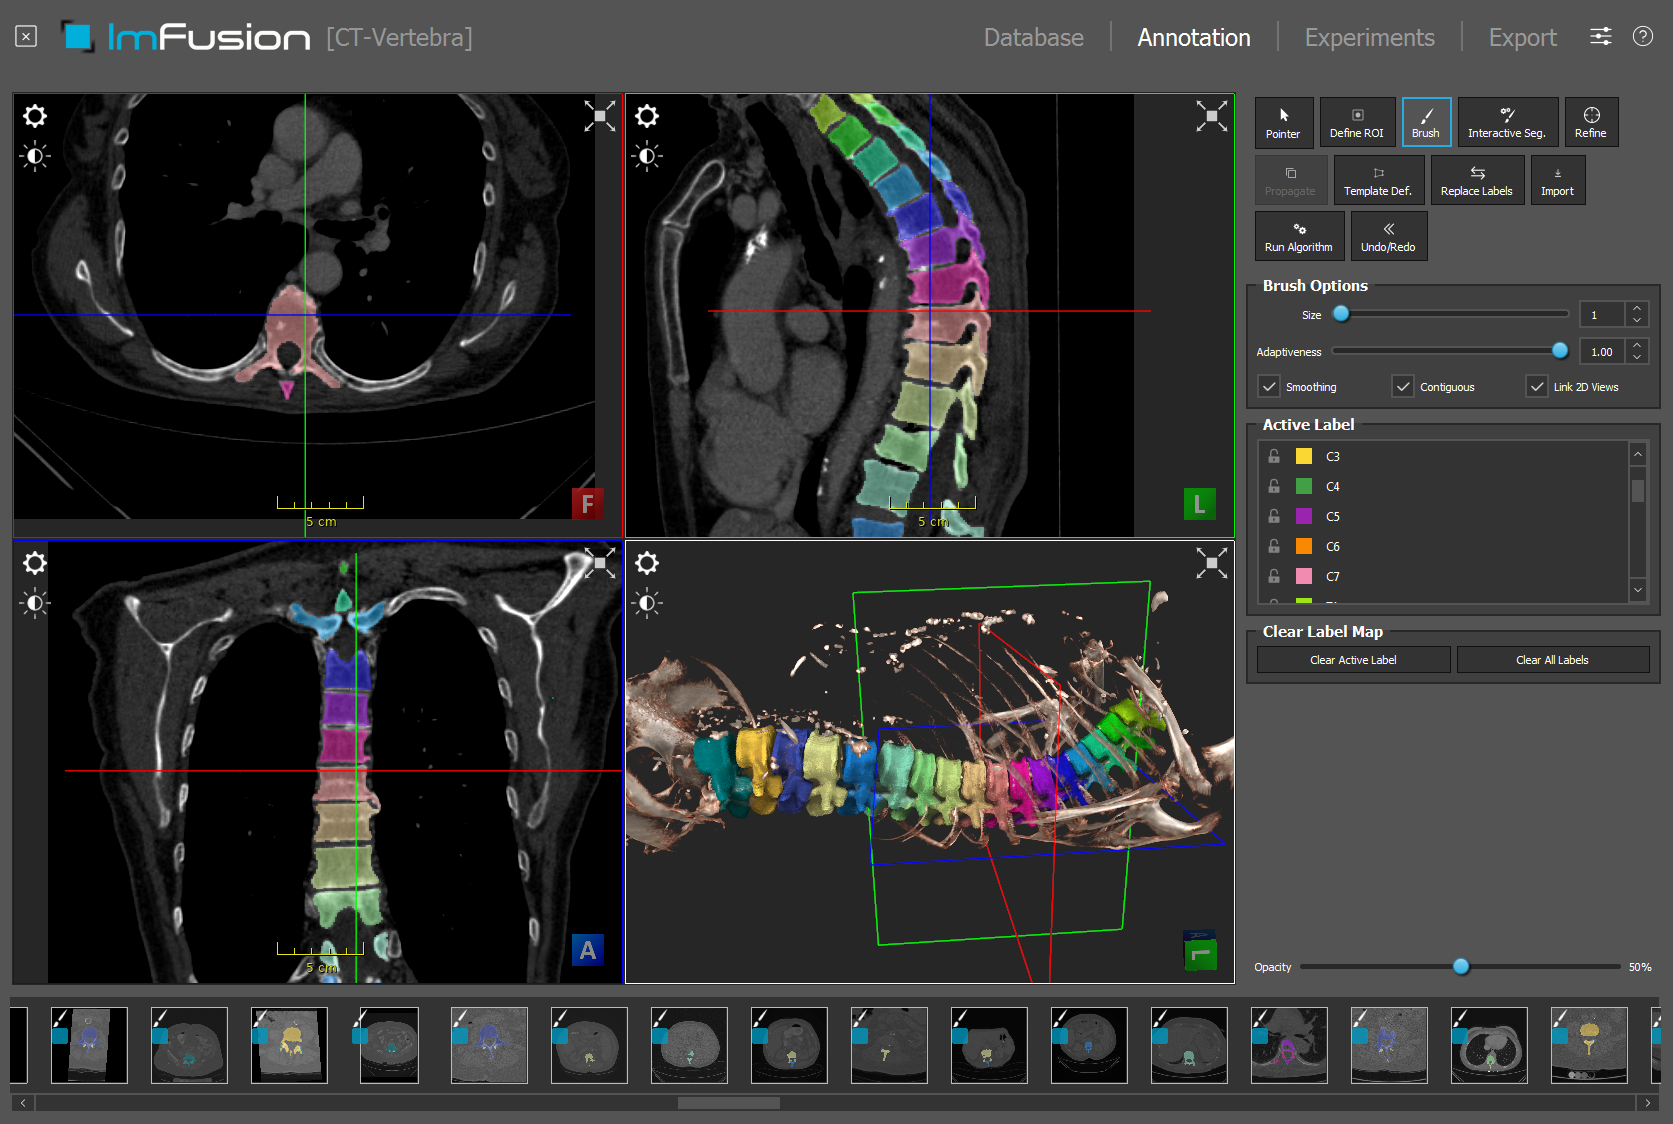
\includegraphics[width=2.5cm]{./images/imfusion_picture_00.png}};
		\node[anchor=north west] (box) at (a.north east) {
			\parbox{10cm}{%
				\begin{itemize}
					\item[{
\includegraphics[height=1.5ex]{./images/icon_place.png}}] Founded: 2012 | Location: Munich, Germany
					\item[{
\includegraphics[height=1.5ex]{./images/icon_flask.png}}] Private \& Independent R\&D Lab
					\item[{
\includegraphics[height=1.5ex]{./images/icon_handshake.png}}] Software framework: trusted by industry leaders, start-ups, and research labs
					\item[{
\includegraphics[height=1.5ex]{./images/icon_glass.png}}] Academic engagement: Actively contributing to the research community
					\item[{
\includegraphics[height=1.5ex]{./images/icon_group.png}}] Our team:
					\begin{itemize}
						\item 50+ dedicated employees and several students
						\item Global Diversity: 10+ Nationalities
						\item Excellence in Expertise: 50\% of technical staff hold a PhD
						\item Groups: Core, Computer Vision, Machine Learning, Ultrasound, CT \& Interventional X-Ray, Robotics.
					\end{itemize}
				\end{itemize}
			}
		};
		\node[anchor=north] at (a.south) {
			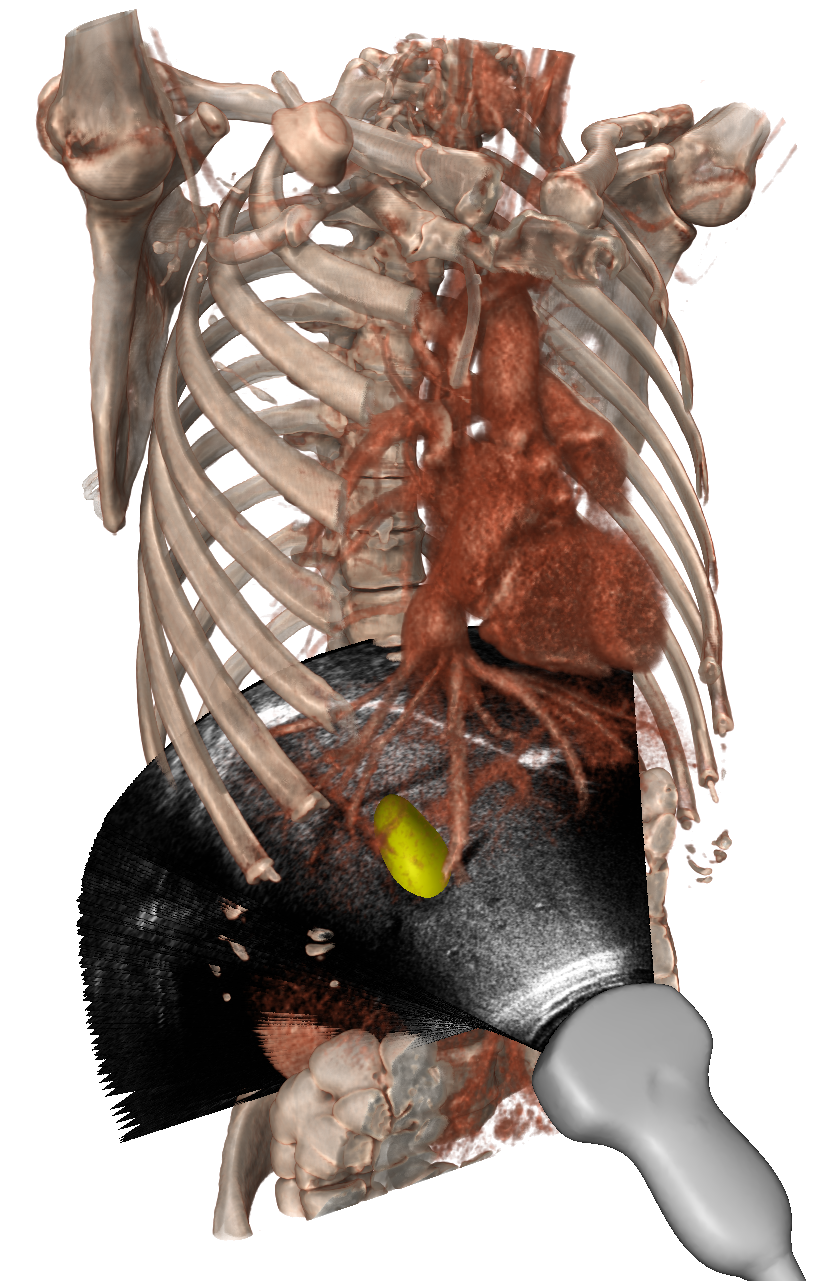
\includegraphics[width=2.5cm]{./images/imfusion_picture_01.png}};
		\node[anchor=north west] at (box.north east) {
			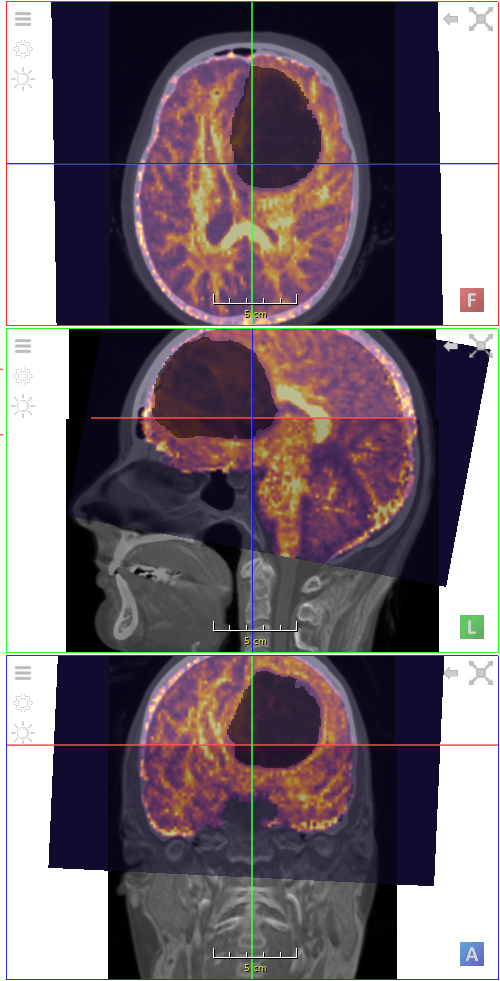
\includegraphics[width=2.5cm]{./images/imfusion_picture_02.png}};
	\end{tikzpicture}
\end{frame}

\begin{frame}[t]
	\frametitle{Robotics}
	\hglue -1cm
	\begin{tikzpicture}[scale=1, transform shape]
		\node (a) {
			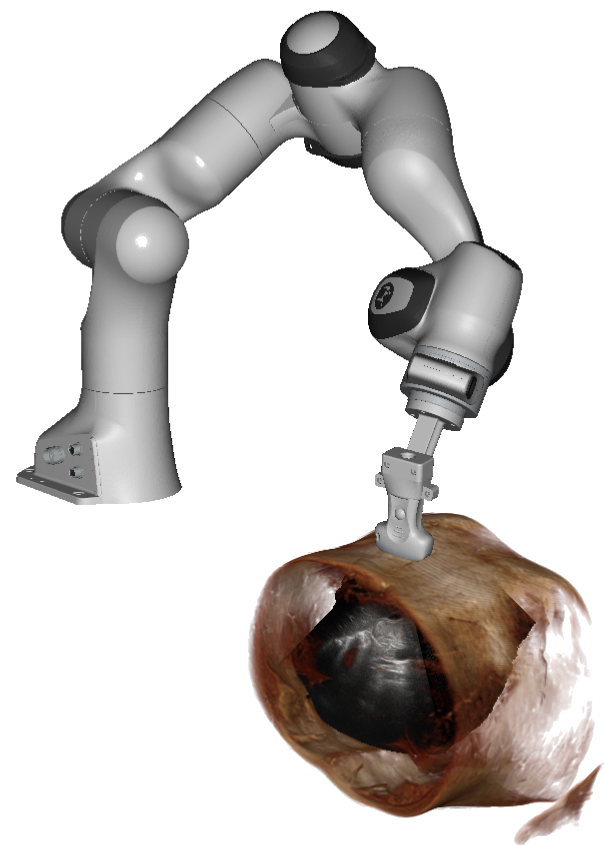
\includegraphics[width=3.4cm]{./images/imfusion_picture_03.png}};
		\node[anchor=north] at (a.south) {
			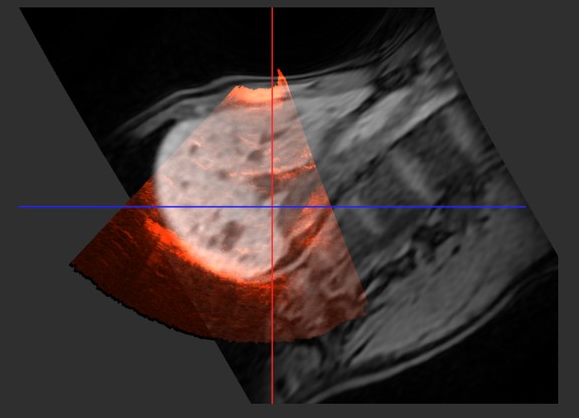
\includegraphics[width=3.4cm]{./images/imfusion_picture_04.png}};
		\node[anchor=north west] (box) at (a.north east) {
			\parbox{10cm}{%
				\begin{itemize}
					\item Deep integration with our framework for surgical navigation, freehand ultrasound, RGBD reconstruction, and more.
					\item Native support for popular robots: Franka Panda, Universal Robot UR-e series, Kuka
					\item Advanced utilities for key use cases: hand-eye calibration, object tracking, telerobotics, custom control strategies.
				\end{itemize}
			}
		};
	\end{tikzpicture}
\end{frame}
